% !TEX TS-program = pdflatexmk
% mnras_template.tex
%
% LaTeX template for creating an MNRAS paper
%
% v3.0 released 14 May 2015
% (version numbers match those of mnras.cls)
%
% Copyright (C) Royal Astronomical Society 2015
% Authors:
% Keith T. Smith (Royal Astronomical Society)

% Change log
%
% v3.0 May 2015
%    Renamed to match the new package name
%    Version number matches mnras.cls
%    A few minor tweaks to wording
% v1.0 September 2013
%    Beta testing only - never publicly released
%    First version: a simple (ish) template for creating an MNRAS paper

%%%%%%%%%%%%%%%%%%%%%%%%%%%%%%%%%%%%%%%%%%%%%%%%%%

\documentclass[a4paper,fleqn,usenatbib]{mnras}

\usepackage{newtxtext,newtxmath}
\usepackage[T1]{fontenc}
\usepackage{ae,aecompl}
\usepackage{graphicx}	% Including figure files
\usepackage{amsmath}	% Advanced maths commands
\usepackage{amssymb}	% Extra maths symbols
\usepackage{bm}

\newcommand{\nb}{n_{\rm b}}
\newcommand{\prob}{{\rm P}}
\newcommand{\normal}{{\rm{N}}}
\newcommand{\uniform}{{\rm U}}
\newcommand{\dirichlet}{{\rm D}}
\newcommand{\invwish}{{\rm W}^{-1}}
\newcommand{\alphas}{{\bm a}}
\newcommand{\specmean}{{\bm m}}
\newcommand{\speccov}{{\bm S}}
\newcommand{\classprob}{{p}}
\newcommand{\classprobs}{{\bm p}}
\newcommand{\objspec}{{\bm s}}
\newcommand{\objclass}{{\kappa}}
\newcommand{\objclasses}{{\bm \kappa}}
\newcommand{\objdata}{\hat{\bm d}}
\newcommand{\objnoise}{{\bm N}}
\newcommand{\scalemat}{{\bm \Gamma}}
\newcommand{\wfmean}{{\bm w}}
\newcommand{\wfcov}{{\bm W}}

%Editing commands
\newcommand{\bdw}[1]{\textbf{\textcolor{magenta}{BDW: #1}}}

%%%%%%%%%%%%%%%%%%%%%%%%%%%%%%%%%%%%%%%%%%%%%%%%%%

\title[Gaussian Process Spectra]{Gaussian Process Spectra}
\author[S. M. Feeney et al.]{
Stephen M. Feeney,$^{1}$\thanks{E-mail: sfeeney@flatironinstitute.org}
Benjamin D. Wandelt,$^{1,2,3,4}$
and Melissa K. Ness$^{1,5}$
\\
$^{1}$Center for Computational Astrophysics, Flatiron Institute, 162 Fifth Avenue, New York, NY 10010, USA\\
$^{2}$Sorbonne Universit\'e, CNRS, UMR 7095,  Institut d'Astrophysique de Paris (IAP), 98 bis boulevard Arago, 75014 Paris, France\\
$^{3}$Sorbonne Universit\'e, Institut Lagrange de Paris (ILP), 98 bis boulevard Arago, 75014 Paris, France\\
$^{4}$Department of Physics and Astronomy, University of Illinois at Urbana-Champaign, 1002 W Green St, Urbana, IL 61801, USA\\
$^{5}$Department of Astronomy, Columbia University, Pupin Physics Laboratories, New York, NY 10027, USA
}

% These dates will be filled out by the publisher
\date{Accepted XXX. Received YYY; in original form ZZZ}

% Enter the current year, for the copyright statements etc.
\pubyear{2019}

% Don't change these lines
\begin{document}
\label{firstpage}
\pagerange{\pageref{firstpage}--\pageref{lastpage}}
\maketitle

% Abstract of the paper
\begin{abstract}
This is a simple template for authors to write new MNRAS papers.
The abstract should briefly describe the aims, methods, and main results of the paper.
It should be a single paragraph not more than 250 words (200 words for Letters).
No references should appear in the abstract.
Context:
Aims: 
Methods:
Results: 
Conclusions :
\end{abstract}

% Select between one and six entries from the list of approved keywords.
% Don't make up new ones.
\begin{keywords}
keyword1 -- keyword2 -- keyword3
\end{keywords}

%%%%%%%%%%%%%%%%%%%%%%%%%%%%%%%%%%%%%%%%%%%%%%%%%%

\section{Introduction}

[Motivations/goals.] 


There is now a vast set of spectroscopic data and associated label data from surveys like APOGEE, GALAH, LAMOST, SEGUE and RAVE and an increasing number of large spectroscopic surveys will be starting observations in the coming years such as Sloan V, WEAVE, 4 MOST and Gaia RVS. Surveys like GALAH and APOGEE have revolutionised our empirical characterisation of the Milky Way and improved our understanding of its assembly, but both rely on expensive observations integrating to high signal to noise (up to SNR $>$ 100 per pixel) in the pursuit of precision abundances to provide optimal chemical differentiation across the sky (e.g. link to chemical tagging work). Surveys like Sloan V are obtaining an order of magnitude more stars via more efficient sky sampling and by relaxing the SNR limit to ~ 40 per pixel, yet at what precision expense in the derived labels like abundances? Furthermore, GAIA will deliver medium resolution spectra for 7 million objects, with N percent of this being at prohibitive signal to noise for abundance measurements given traditional approaches. There has been to date little characterisation of the true dimensionality and information content of the data. While surveys optimise their wavelength regions to attain an optimal number of element absorption features from which to make measurements, and aim for high signal to noise data, empirically the relationship between signal to noise, precision and information gain across a given wavelength region at a given resolution is unknown. Furthermore it is becoming clear that individual abundances can be measured from their impact on the entire spectral range (Ting 2018) and that precision abundances can be derived from very low resolution spectra (Ho et al., 2016). 
We are therefore at a point where we must assess what the information content of the spectral data actually is, and what expectations of  precision measurements we can make of the data, using automated and data-driven modeling techniques. What is empirically gained by adding an additional element of the same or different nucleosynthetic family in terms of additional spectral information? How correlated or anti-correlated are different spectral features in the data? With respect to the signal to noise required for precision abundance measurements, data-driven modeling like The Cannon and also The Payne have shown that the same precision can be obtained for APOGEE data with 1/4 to 1/9th of the observing time (1/2 to 1/3 of the SNR, so a SNR of around 40 compared to 100 for most abundances) and a precision near the theoretical limit (kramer-rao bound) can be obtained for APOGEE around a SNR of 40 (check), for most elements, which has motivated surveys like Sloan V to optimise their numbers of stars by collecting lower SNR data. Here we expand the 
examination of what information is in stellar spectra from an empirical standpoint. We investigate modeling the APOGEE spectral region using a Gaussian Process, creating a generative model which is an effective de-noising of the individual spectra, that can predict masked or missing spectral regions. We examine in detail the correlations between spectral pixels in element windows and the relative information gain attained by iterative abundance measurements. 

Our approach effectively pools information about stars. In doing this we can: 
% reorder this 
%1. correlations
%2. iformation content
%3. masked regions
%4. make a metric to demonstrate - denoised spectra so can quantify in a section In terms of variances []
%ratio of standard deviations of the pink to the grey
\begin{enumerate}
\item Predict masked (unmeasured or contaminated) regions of the spectra to make, e.g., abundance measurements that would otherwise be impossible. This may be particularly valuable in APOGEE for r-process element measurements where only one or two features exist from which to make measurements where this valuable element adds the dimensionality of the neturon-capture nucleosynthetic family [Section 2], or elements or features near the chip gaps that are present in some spectra and not others due to stellar velocities (citation. [Section 1] 
\item Examine in detail the empirical correlations in the spectra, make quantitative measurements of these correlations and identify in practice which elements are positively and which are negatively affiliated. [Section 2: might just want to add a plot of which are + and which are - correlated] 
\item Denoise to make precision measurements at lower SNR.  Generically, we can use the data-driven GP mixture model to denoise and thus enhance the data, potentially enabling new discoveries. This should work for high S/N and low S/N regions; how useful this is depends on the size of the effects we may want to discover. Our expectation is that this is particulalry good for very weak features such as (Hasselquist) expectation is can do a lot better with abundance measurements, similarly to that previously demonstrated with generative modeling (The Cannon, The Payne). 
\item Determine the most informative regions of spectra and make a measure of the information content of the data to, e.g., determine whether we can retain sensitivity to abundances by observing a reduced spectral range and to understand if we have a set of N elements measured, do we gain information empirically by moving to N+1 measurements, for different element combinations, at the SNR of the APOGEE data. 
\end{enumerate}

%Is there any purpose of measuring all these elements? Empirically extra information in them? 

%-first look at the information content of the spectra
%-first characterisation and mapping of the element correlations

%state just red clump sample 

%[Ce, Cu, Mg, Ni, Mn, N, C, Ti, Si, Mg, Na, Fe, O, Ti, Ca, Nd, Fe, Si, Mn, Al, N, Ni, C]
%light: C, N
%light odd-Z: Na, Al
%alpha: Mg, Ti, Si, O
%iron-peak: Cu, Ni, Mn, Fe
%neutron capture r-process: Ce, Nd



%Fig 4 - trying to bring out the correlation structure in a slightly different way

%Fig 4 - perfectly uncorrelated would be random purpose and yellow because none of the pixels in the bin compare about any of the pixels in any other bin. If perfectly correlated yellow all up the top, purple all down the bottom. 

%-not parameterised in any physical way
%understanding of stellar spectra is truly rudimentary 
%this is part of a bigger effort in order to (under the assumption that everything is Guassian) allows us to learn the covariance at every point completely independent of any given physical template. 
%- question about the degrees of freedom (N*N)/2 degrees of freedom, diagonal of the covariance matrix
%- big thing is it shows the covariances
%-understand what the information content of the spectra%
%-inferring true spectra of every star.( N*N + Nclasses*2 + N*N)/2
%in the context of a much more sophistocated model 
%-runs into problems as matrix algebra (just gets really slow) 
%-new things
%-can do de-noising 

%Fig 6: information gain for each element and then pick the one that is most informative and then calculate the information gain on the window of interest given most informative element and each other one
%-log of the determinant of the covariance matrix of the window/ log of the covariance matrix of the window conditioned on other data
%-



%to do: For the Figure 6 - a list of the windows and the element families and then that is a whole little section . 

%Fig 2 - go down to just the window

%Fig 5: corner put SNR 

%state just red clump sample 

%How will we do this? By modeling the spectra as a data-driven Gaussian Process. What is a GP and what are relevant applications.

%%%%%%%%%%%%%%%%%%%%%%%%%%%%%%%%%%%%%%%%%%%%%%%%%%




\section{Data} 

For our modeling we use the APOGEE red clump spectra from DR14 (cite Majewski, and Bovy 2014). These spectra comprise $29502$ stars with a mean SNR of XX and range of SNR of 20-XX.  The contamination of red giant stars within this sample is on the order of 5-20 percent (Bovy, Ting).  These make an ideal test case for our modeling being restricted in their range of effective temperature and surface gravity so we can assume that our overall measurements are driven by abundance variations and not systematic variations across stellar parameters. The metallicity range of the red clump stars span --1.0 $<$ [Fe/H] $<$ 0.5 and they are distributed from R$_{GAL}$ = 4 to 20 kpc. 


The data have been downloaded from the APOGEE database and come radial velocity shifted and continuum-normalised (with a slight SNR dependence on the continuum normalisation that we discover with our Gaussian Process modeling. The spectra cover the range 15100.80-16999.81 \AA, using $\nb = 8575$ spectral bins. 

\section{Methods}

Describe Gaussian Process. True spectrum for each star is drawn from a GP with a mean spectrum and covariance matrix to be inferred from the data. We do not assume a kernel for our GP covariance, but rather infer the correlations between the observed spectral bins. This is so we can model the exact covariance and not worry about suboptimal choices of kernels caused by non-stationarity or different correlation lengths, line shapes, etc. The main downside of doing this is we can not make predictions for the spectra between the observed bins, though we could, given data observed on shifted or irregularly or different-spaced grids. We assume uninformative priors on the mean and covariance. We adopt an infinite uniform prior on the mean and a Jeffreys prior on the covariance matrix (precise form in notes).

Data are observed with Gaussian noise that is uncorrelated between spectral bins; masked pixels are assigned unit flux and effectively infinite noise uncertainties. These data, the inferred parameters, the likelihood and priors would fully specify the model if we had only one class. To account for the fact that the red clump might consist of multiple distinct populations (or one population whose distribution of true spectra is non-Gaussian) we allow for multiple classes to exist in our model. In this instance, each star is also assigned membership to a particular class. Class memberships are drawn from categorical distributions, with class probabilities drawn from a symmetric Dirichlet prior with concentration parameter $\alpha=1$.

The network diagram for our hierarchical Bayesian model is shown in Fig.~\ref{fig:network_diagram}, and the probability distributions defining each link are set out in Table.~\ref{tab:prob_dists}. The particular set of probability distributions chosen allow for the conditional distributions of each latent variable to be written analytically, and we hence use Gibbs sampling to estimate the joint posterior.

\begin{figure}
	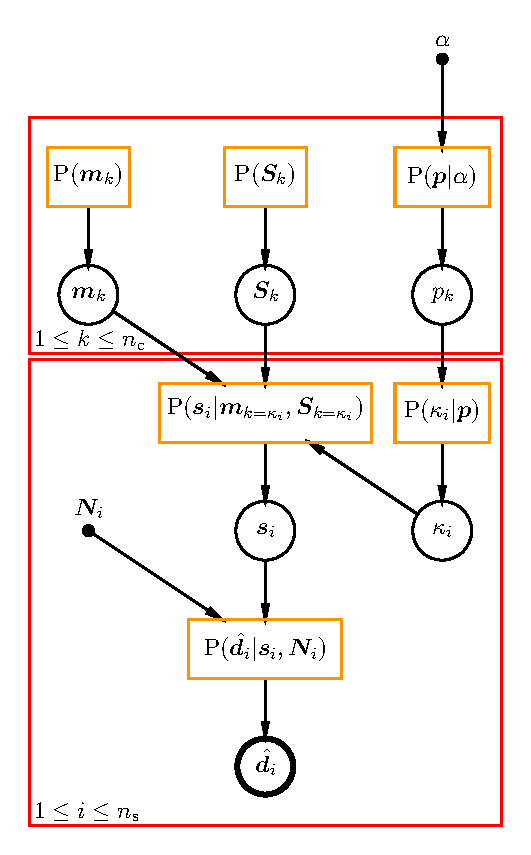
\includegraphics[width=\columnwidth]{bhm_plot.pdf}
    \caption{Network diagram for our hierarchical Bayesian model.}
    \label{fig:network_diagram}
\end{figure}

\begin{table*}
    \centering
    \caption{Priors, likelihoods and conditional distributions for Gibbs sampling. In our simplified notation, $\uniform$, $\dirichlet$, $\normal$ and $\invwish$ denote uniform, Dirichlet, normal and inverse-Wishart distributions, respectively.}
    \label{tab:prob_dists}
    \begin{tabular}{lll}
        \hline
        distribution & form & process \\
        \hline
        $\prob\left(\specmean_k\right)$ & $\uniform\left(-\infty,\infty\right)$ & Prior on $k^{\rm th}$ class's mean spectrum \\
        $\prob\left(\speccov_k\right)$ & $\left| \speccov \right|^{-\left(\nb+1\right)/2}$ & Prior on $k^{\rm th}$ class's spectrum covariance \\
        $\prob\left(\classprobs|\alpha\right)$ & $\dirichlet\left(\alpha\right)$ & Prior on class probabilities \\
        $\prob\left(\objspec_i|\specmean,\speccov,\objclass_i\right)$ & $\normal\left(\specmean_{k=\objclass_i},\speccov_{k=\objclass_i}\right)$ & $i^{\rm th}$ object's spectrum as Gaussian Process \\
        $\prob\left(\objclass_i = k|\classprobs\right)$ & $\classprob_k$ & $i^{\rm th}$ object's class membership \\
        $\prob\left(\objdata_i|\objspec_i,\objnoise_i\right)$ & $\normal\left(\objspec_i,\objnoise_i\right)$ & Noisy, masked spectral measurements \\
        \hline
        $\prob\left(\specmean_k | \speccov_k, \objspec, \objclasses \right)$ & $\normal \left( \frac{1}{n_k} \sum_{\objclass_i = k} \objspec_i, \frac{1}{n_k} \speccov_k \right)$ & Conditional on $k^{\rm th}$ class's mean spectrum \\
%        $\prob\left(\speccov_k | \specmean_k, \objspec, \objclasses \right)$ & $\left| \speccov_k \right|^{-(n_k + \nb + 1)/2} \exp \left( -\frac{1}{2} {\rm tr} \left[ \scalemat_k \speccov_k^{-1} \right] \right)$, where & Conditional on $k^{\rm th}$ class's spectrum covariance \\
        $\prob\left(\speccov_k | \specmean_k, \objspec, \objclasses \right)$ & $\invwish \left(n_k, \scalemat_k \right)$, & Conditional on $k^{\rm th}$ class's spectrum covariance \\
         & where  $\scalemat_k = \sum_{\objclass_i = k} \left( \objspec_i - \specmean_k \right) \otimes \left( \objspec_i - \specmean_k \right)$ & \\
        $\prob\left(\classprob_k | \objclasses, \alpha\right)$ & $\dirichlet\left(\alphas\right)$, where $a_k = \alpha + n_k$ & Conditional on class probabilities \\
        $\prob \left( \objspec_i | \specmean_{k=\objclass_i}, \speccov_{k=\objclass_i}, \objdata_i, \objnoise_i \right)$ & $\normal \left( \wfmean_i, \wfcov_i \right)$, & Conditional on $i^{\rm th}$ object's spectrum \\
         & where $\wfcov_i = \left( \speccov_{k=\objclass_i}^{-1} + \objnoise_i^{-1} \right)^{-1}$ &  \\
         & and $\wfmean_i = \wfcov_i \left( \speccov_{k=\objclass_i}^{-1} \specmean_{k=\objclass_i} + \objnoise_i^{-1} \objdata_i \right)$ &  \\
        $\prob \left( \objclass_i = k | \specmean, \speccov, \classprobs \right)$ & $ \frac{ \exp \left( -\frac{1}{2} \left[ \chi^2_{i,k} + \ln \left| \speccov_k \right| \right] + \ln \classprob_k \right) }{ \sum_{k^\prime} \exp \left( -\frac{1}{2} \left[ \chi^2_{i,k^\prime} + \ln \left| \speccov_{k^\prime} \right| \right] + \ln \classprob_{k^\prime} \right) }$, & Conditional on $i^{\rm th}$ object's class membership \\
         & where $\chi^2_{i,k} = \left( \objspec_i - \specmean_k \right)^T \speccov_k^{-1} \left( \objspec_i - \specmean_k \right) $ &  \\
        \hline
    \end{tabular}
\end{table*}

%%%%%%%%%%%%%%%%%%%%%%%%%%%%%%%%%%%%%%%%%%%%%%%%%%

We take the 29502 red clump stars identified in the APOGEE dataset with their 8575 pixels over the spectral range 15100.80-16999.81 \AA, using $\nb = 8575$ spectral bins. Inversion of the resulting $\nb \times \nb$ covariance matrices would be too slow to permit inference, and we thus restrict our analysis to a set of spectral windows centred on lines confidently assigned to individual elements. These element windows have been chosen from the set of windows used to drive the APOGEE abundances (described in citation). Specifically, we process all spectral bins within $\pm2.5$ \AA\ of the line centres tabulated in Table~\ref{tab:window_centres}, reducing the number of spectral bins to $\nb = 557$ and hence inversion time by a factor of $\sim3500$.

\begin{table}
    \centering
    \caption{Elemental windows.}
    \label{tab:window_centres}
    \begin{tabular}{lcc}
        \hline
        element & window & window \\
         & centre 1 & centre 2 \\
        \hline
        Al & 15972.905 & - \\
        C & 15479.107 & 15582.101 \\
        Ca & 16161.807 & - \\
        Cu & 16010.023 & - \\
        Fe & 15494.733 & 15505.643 \\
        Mg & 15425.309 & 15697.701 \\
        Mn & 15162.885 & 15221.867 \\
        N & 15161.42 & 15321.871 \\
        Na & 16393.443 & - \\
        Ni & 15559.517 & 15758.315 \\
        O & 15269.893 & 15631.468 \\
        Si & 15365.335 & 15964.753 \\
        Ti & 15190.779 & 15339.241 \\
        Ce & 15789.063 & 16380.954 \\
        Nd & 16058.014 & - \\
        \hline
    \end{tabular}
\end{table}

%%%%%%%%%%%%%%%%%%%%%%%%%%%%%%%%%%%%%%%%%%%%%%%%%%

\section{Results}

\subsection{Validation of Methodology: Predicting Unmeasured Spectral Regions}

To avoid the complications of comparing data gathered by different spectrographs we validate our model and code by artificially masking a portion of one of our APOGEE spectra, namely the 15789 \AA\ Cerium window of our lowest-SNR star (2M18335753-1302240). The measured data for this star are plotted in Figure~\ref{fig:recovery_test} as a solid black line, with the artificially masked region picked out as a dashed line. The 68\% credible interval for the posterior probability on the star's true spectrum is plotted as dark grey, with the corresponding prediction for the observed spectrum (which also takes into account the uncertainty on the observations) plotted in light grey. This prediction (the posterior predictive distribution of the measured data) is in excellent agreement with the measured data, indicating that our model is capable of inpainting masked regions without bias. Note, in addition, that the uncertainty on the true spectrum is much smaller than the measurement noise, demonstrating our method's ability to denoise observed spectra.

\begin{figure}
	\includegraphics[width=\columnwidth]{apogee_centers_subset2_ce_nd_29502_spc_rec_test_recovery_zoom.pdf}
    \caption{\textcolor{red}{[Remove the side regions, just show the Cerium window.]}Recovery test. Artificially masking the 15789 \AA\ Cerium window (indicated by vertical dotted lines) for the lowest-SNR star results in an inferred true spectrum (dark-grey shaded region) that is entirely in agreement with the measurement (solid black line) once noise is taken into account (light-grey shaded region).}
    \label{fig:recovery_test}
\end{figure}

\subsection{APOGEE Inference: Feature Correlations Across the Abundance Windows}


Our inference produces samples of the probability, mean spectrum and covariance matrix for each class considered, and the true spectrum and class membership of each object. Focusing initially on the single-class case, we plot our covariance and mean inference in Figures~\ref{fig:inferred_cov} and~\ref{fig:gp_reals}, respectively. We plot the mean-posterior covariance matrix in Figure~\ref{fig:inferred_cov} (left panel). The covariance has strong off-diagonal structure, indicating that certain spectral features are highly correlated and anti-correlated ({\bf discuss potential kernel choices?}). Its eigenspectrum also decays rapidly: only 241 of 557 eigenmodes have eigenvalues larger than 1/100 of the maximum. A low-rank approximation to the mean covariance retaining only these eigenmodes is plotted in the centre panel of Figure~\ref{fig:inferred_cov}, and the resulting residuals (multiplied by a factor of 500 to render visible) in the right panel. Exploiting this decaying eigenspectrum by assuming the covariance is rank deficient would greatly reduce computation time (by a factor of roughly 12 if 241 modes were retained). Na\"ively projecting the data onto the largest principal components of the sample covariance matrix prior to inference severely degrades performance. Modifying the hierarchical model (along the lines of {\bf citations}) to explicitly infer a rank-deficient covariance matrix is left to future work.

\begin{figure*}
	\includegraphics[width=2\columnwidth]{apogee_centers_subset2_ce_nd_29502_spc_low_rank_covariance.pdf}
    \caption{Mean-posterior covariance matrix (left), its low-rank approximation (centre) constructed from all eigenvectors with eigenvalues within $10^{-4}$ of the largest, and the residuals (right). \textcolor{red}{[This Figure demonstrates that the spectral pixels are highly correlated. If uncorrelated would expect purely white and if perfectly correlated would expect blue and red (positive and negative correlations respectively).]}}
    \label{fig:inferred_cov}
\end{figure*}

\begin{figure*}
	\includegraphics[width=2\columnwidth]{apogee_centers_subset2_ce_nd_29502_spc_gp_realizations.pdf}
    \caption{Mean-posterior mean spectrum (black), and 50 realizations drawn from our Gaussian Process model, conditioned on the APOGEE data, coloured purple to yellow according to their flux in the first spectral bin.\textcolor{red}{ [Add to caption very explicit that this is another visualisation to complement Figure 3, about how strongly correlated everything is. If was purple to yellow clearly everything entirely correlated, if no structure in colour entirely uncorrelated.]  }}
    \label{fig:gp_reals}
\end{figure*}

The posterior mean of the mean spectrum is plotted in black in Figure~\ref{fig:gp_reals}. The mean spectrum is extremely well constrained: its 68\% credible interval is narrower than the width of line. To illustrate the covariance structure captured by our model, we overlay 50 realizations drawn from our Gaussian-Process model conditioned on the APOGEE data, colour-coded by the value they take in the first spectral bin. These samples can be interpreted as examples of potential noiseless true spectra that could have led to the data. They illustrate the variability permitted by the model and highlight certain clear trends, most notably highly correlated differences in line depths.

We demonstrate our inference of the true spectra of individual stars in Figure~\ref{fig:inpainting_denoising_examples}, selecting six illustrative examples. From top to bottom, we pick out two spectra whose 15789 \AA\ Cerium windows are completely masked; two spectra whose 16058 \AA\ Neodymium windows are fully masked; and the two lowest signal-to-noise spectra. The APOGEE IDs for these stars are 2M00014650+7009328, 2M00031631+0042234, 2M00184317+5821021, 2M03320729+4526557, 2M18335753-1302240 and 2M18295507-0340512, with signal-to-noise ratios of 49, 63, 480, 1116, 21 and 23. Each panel of Figure~\ref{fig:inpainting_denoising_examples} contains two shaded regions. The pink shaded area indicates the one-sigma deviations from the measured spectra due to noise (these are infinitely wide when the spectrum is masked); the grey, the 68\% posterior credible intervals on the true spectra. Recall that we are inferring the true spectra only at the measured spectral bins only. In this sense the smooth grey curves are perhaps misleading, as the posterior uncertainty is strictly infinite between datapoints.
 
true spectra. fit to observations. inpainting, denoising. quantify? any underperformance? Ni band of star 2. N/Mn (and Ti) bin of lowest SNR star (and 2nd lowest?).
number of classes, high-dim inference

\begin{figure*}
	\includegraphics[width=2\columnwidth]{apogee_centers_subset2_ce_nd_29502_spc_save_spectra.pdf}
    \caption{Observed spectra (pink shaded regions) and inferred ``true'' spectra (grey shaded regions) for six interesting examples illustrating our ability to inpaint and denoise. From top: two spectra with the 15789 \AA\ Cerium window fully masked; two spectra with the 16058 \AA\ Neodymium window fully masked; the two lowest signal-to-noise spectra. \textcolor{red}{put SNR in corner of each}}
    \label{fig:inpainting_denoising_examples}
\end{figure*}

\subsection{The Measured Information Content in the Spectra}

predictivity
Here we measure information gain. Given one element, how much information do we gain by measuring one more element, and then another. 
Demonstrate for each family
Metric is this: 
What we find is essentially every single element adds information. Flat line would indicate no additional information, falls of exponentially at different rates for all the elements. Log scale so fractional gain for first N elements is XX and fractional gain for elements $>$ 5 is XX percent, relatively independent of which element is conditioned on. 

\begin{figure*}
	\includegraphics[width=2\columnwidth]{apogee_centers_subset2_ce_nd_29502_spc_ce_inf_gain.pdf}
	\includegraphics[width=2\columnwidth]{apogee_centers_subset2_ce_nd_29502_spc_ce_conditional_stddevs.pdf}
    \caption{\textcolor{red}{[do for each family with a sample element and color families together (see email) ]} Information gain (top) and conditional standard deviation (bottom) for Cerium windows given observations of other elemental windows. The uncertainty on the predicted spectrum without observations of other windows is shown in black\bdw{Is this the same as the noise?}.}
    \label{fig:ce_information}
\end{figure*}

\begin{figure}
	\includegraphics[width=\columnwidth]{apogee_centers_subset2_ce_nd_29502_spc_nd_inf_gain.pdf}
	\includegraphics[width=\columnwidth]{apogee_centers_subset2_ce_nd_29502_spc_nd_conditional_stddevs.pdf}
    \caption{Information gain (top) and conditional standard deviation (bottom) for Neodymium window given observations of other elemental windows. The uncertainty on the predicted spectrum without observations of other windows is shown in black.}
    \label{fig:nd_information}
\end{figure}



%%%%%%%%%%%%%%%%%%%%%%%%%%%%%%%%%%%%%%%%%%%%%%%%%%

\section{Conclusions}

TBD.

%%%%%%%%%%%%%%%%%%%%%%%%%%%%%%%%%%%%%%%%%%%%%%%%%%

\section*{Acknowledgements}

The Flatiron Institute is supported by the Simons Foundation.

%%%%%%%%%%%%%%%%%%%%%%%%%%%%%%%%%%%%%%%%%%%%%%%%%%

%\bibliographystyle{mnras}
%\bibliography{example} % if your bibtex file is called example.bib

%%%%%%%%%%%%%%%%%%%%%%%%%%%%%%%%%%%%%%%%%%%%%%%%%%


% Don't change these lines
\bsp	% typesetting comment
\label{lastpage}
\end{document}

% End of mnras_template.tex